\documentclass[12pt]{beamer}
\newenvironment{ConCodigo}[1]
  {\begin{frame}[fragile,environment=ConCodigo]{#1}}
  {\end{frame}}
\graphicspath{{Imagenes/}{../Imagenes/}}
\usepackage[utf8]{inputenc}
\usepackage[spanish]{babel}
\usepackage{hyperref}
\usepackage{etex}
%\reserveinserts{28}
\usepackage{amsmath}
\usepackage{amsthm}
\usepackage{mathtools}
\usepackage{multicol}
\usepackage{multirow}
\usepackage{tabulary}
\usepackage{booktabs}
\usepackage{nccmath}
\usepackage{physics}
\usepackage{biblatex}
\usepackage[outdir=./]{epstopdf}
%\epstopdfsetup{outdir=./}
\usepackage{graphicx}
%\usepackage{enumitem,xcolor}
\usepackage{siunitx}
%\sisetup{scientific-notation=true}
%\usepackage{fontspec}
\usepackage{lmodern}
\usepackage{float}
\usepackage[format=hang, font=footnotesize, labelformat=parens]{caption}
\usepackage[autostyle,spanish=mexican]{csquotes}
\usepackage{standalone}
\usepackage{blkarray}
\usepackage{algorithm}
\usepackage{algorithmic}
\usepackage{tikz}
\usepackage[siunitx, RPvoltages]{circuitikz}
\usetikzlibrary{arrows,patterns,shapes}
\usetikzlibrary{decorations.markings}
\usetikzlibrary{arrows}
\usepackage{color}
\usepackage{xcolor}
%\usepackage{beton}
%\usepackage{euler}
%\usepackage[T1]{fontenc}
\usepackage[sfdefault]{roboto}  %% Option 'sfdefault' only if the base font of the document is to be sans serif
\usepackage[T1]{fontenc}
\renewcommand*\familydefault{\sfdefault}
\DeclareGraphicsExtensions{.pdf,.png,.jpg}
\usepackage{hyperref}
\renewcommand {\arraystretch}{1.5}
\newcommand{\python}{\texttt{python}}
\usefonttheme[onlymath]{serif}
\setbeamertemplate{navigation symbols}{}
\usetikzlibrary{patterns}
\usetikzlibrary{decorations.markings}
\tikzstyle{every picture}+=[remember picture,baseline]
%\tikzstyle{every node}+=[inner sep=0pt,anchor=base,
%minimum width=2.2cm,align=center,text depth=.15ex,outer sep=1.5pt]
%\tikzstyle{every path}+=[thick, rounded corners]
\setbeamertemplate{caption}[numbered]
\newcommand{\ptm}{\fontfamily{ptm}\selectfont}
%Se usa la plantilla Warsaw modificada con spruce
\mode<presentation>
{
  \usetheme{Warsaw}
  \setbeamertemplate{headline}{}
  \useoutertheme{default}
  \usecolortheme{albatross}
  \setbeamercovered{invisible}
}
% \AtBeginSection[]
% {
% \begin{frame}<beamer>{Contenido}
% \normalfont\mdseries
% \tableofcontents[currentsection]
% \end{frame}
% }

\include{pre_codigo}
\usepackage{siunitx}
\usepackage[american,cuteinductors,smartlabels]{circuitikz}
\usetikzlibrary{calc}
\title{Ecuaciones diferenciales ordinarias 5}
\subtitle{Curso de F\'{i}sica Computacional}
\author{M. en C. Gustavo Contreras May\'{e}n}
%\date{18 de octubre de 2012}
%\email{curso.fisica.comp@gmail.com}
%\ptsize{10}
\begin{document}
\maketitle
\fontsize{14}{14}\selectfont
\spanishdecimal{.}
\begin{frame}{Contenido}
\tableofcontents[pausesections]
\end{frame}
\section{EDO con valores en las fronteras}
\begin{frame}
\frametitle{EDO con valores en las fronteras}
En lo que hemos visto del tema, recordamos que una EDO se acompaña de condiciones auxiliares. Estas condiciones se usan para evaluar las constantes de integraci\'{o}n que resultan durante la soluci\'{o}n de la ecuaci\'{o}n. Para una ecuaci\'{o}n de $n$-\'{e}simo orden, se requieren $n$ condiciones. Si todas las condiciones se especifican en el mismo valor de la variable independiente, entonces estamos tratando con un problema de valor inicial.
\end{frame}
\begin{frame}
En contraste, hay un conjunto de problemas en los cuales las condiciones no son conocidas en un solo punto, sino, m\'{a}s bien, son conocidas en diferentes valores de la variable independiente.
\\
\bigskip
Como estos valores se especifican a menudo en los puntos extremos o fronteras de un sistema, se les conoce como problemas de valores en la frontera.
\end{frame}
\begin{frame}
\frametitle{Ejemplo}
Se puede usar la conservaci\'{o}n de calor para desarrollar un balance de calor para una barra larga y delgada. Si la barra no est\'{a} aislada en toda su longitud y el sistema se encuentra en estado estable, la ecuación resultante es
\begin{equation} \label{eq:ec_calor1}
 \dfrac{d^{2}T}{dx^{2}} + \alpha(T_{a} - T) = 0 
\end{equation}
donde $\alpha$ es un coeficiente de transferencia de calor ($cm^{-2}$) que parametriza la raz\'{o}n de disipaci\'{o}n de calor con el aire circundante, y $T_{a}$ es la temperatura del aire circundante.
\end{frame}
\begin{frame}
\frametitle{Problema de temperatura}
\begin{tikzpicture}[font=\small]
\draw [pattern=north east lines] (-1,-2) rectangle (0,2);
\draw (-1,-2) -- node [midway, left] {$T_{1}$}(-1,2);
\draw (0,-0.5) rectangle (7,0.5);
\draw [pattern=north east lines] (7,-2) rectangle (8,2);
\draw (8,-2) -- node [midway, right] {$T_{2}$}(8,2);
\draw (3.3,1.8) node {$T_{a}$};
\foreach \x in {1cm, 3cm, 5cm}
	\draw [->, thick] (\x,0.7) -- (\x,1.3);
\foreach \x in {1cm, 3cm, 5cm}
	\draw [->, thick] (\x,-0.8) -- (\x,-1.4);
\draw [->, thick] (1,0) -- (6,0);
\draw (-0.1,-2.3) node {x=0};
\draw (7.1,-2.3) node {x=L};
\end{tikzpicture}
\end{frame}
\begin{frame}
Para obtener una soluci\'{o}n para la ecuaci\'{o}n (\ref{eq:ec_calor1}) se deben tener las condiciones en la frontera adecuadas. Un caso simple se presenta donde los valores de las temperaturas en los extremos de la barra se mantienen con valores fijos. Estos valores se pueden
expresar matem\'{a}ticamente como
\[ \begin{split} 
T_{0} =& T_{1} \\
T_{L} =& T_{2}
\end{split} \]
Con estas condiciones, la ecuación (\ref{eq:ec_calor1}) se puede resolver de manera anal\'{i}tica.
\end{frame}
\begin{frame}
Para una barra de 10 metros con $T_{a} = 20$, $T_{1} = 40$, $T_{2} = 200$ y $\alpha = 0.01$, el resultado es
\[ T = 73.4523 \exp(0.1x) - 53.4523 \exp (-0.1x) + 20\]
\end{frame}
\section{El m\'{e}todo de disparo}
\begin{frame}
\frametitle{El m\'{e}todo de disparo}
El m\'{e}todo de disparo se basa en convertir el problema de valor en la frontera en un problema equivalente de valor inicial.
\\
\bigskip
Posteriormente se implementa un procedimiento de prueba y error para resolver la versi\'{o}n de valor inicial. El procedimiento se puede ilustrar con un ejemplo.
\end{frame}
\begin{frame}
\frametitle{Problema}
Utilizando el m\'{e}todo de disparo para resolver la ecuaci\'{o}n (\ref{eq:ec_calor1}), para una barra de 10 metros, con $\alpha= 0.01m^{2}$, $T_{a}=20$, y las condiciones de frontera
\[ \begin{split} 
T(0)=& 0 \\
T(10) =& 200 
\end{split} \]
\end{frame}
\begin{frame}
\frametitle{Soluci\'{o}n}
Transformamos la ecuaci\'{o}n (\ref{eq:ec_calor1}) en dos EDO de primer orden:
\begin{eqnarray*}
\dfrac{dT}{dx} &=& z \\
\dfrac{dz}{dz} &=& \alpha (T - T_{a})
\end{eqnarray*}
Para resolver estas ecuaciones, se requiere un valor inicial para $z$, por el m\'{e}todo de disparo, intuimos un valor, digamos $z(0)=10$. Usando RK4 en las dos ecuaciones obtenemos
\end{frame}
\begin{frame}
\fontsize{12}{12}\selectfont
\begin{center}
\begin{tabular}{c | c | c}
 x & y[0] & y[1] \\ \hline
0.0000e+00 & 4.0000e+01 & 1.0000e+01 \\
1.0000e+00 & 5.0484e+01 & 1.0952e+01 \\
2.0000e+00 & 6.1873e+01 & 1.1813e+01 \\
3.0000e+00 & 7.4082e+01 & 1.2592e+01 \\
4.0000e+00 & 8.7032e+01 & 1.3297e+01 \\
5.0000e+00 & 1.0065e+02 & 1.3935e+01 \\
6.0000e+00 & 1.1488e+02 & 1.4512e+01 \\
7.0000e+00 & 1.2966e+02 & 1.5034e+01 \\
8.0000e+00 & 1.4493e+02 & 1.5507e+01 \\
9.0000e+00 & 1.6066e+02 & 1.5934e+01 \\
1.0000e+01 & 1.7679e+02 & 1.6321e+01
\end{tabular}
\end{center}
\end{frame}
\begin{frame}
\frametitle{Gr\'{a}ficamente con $Z(0)= 10$}
\begin{figure}
	\centering
	\includegraphics[scale=0.5]{MetDisparo01.eps} 
\end{figure}
\end{frame}
\begin{frame}
El resultado obtenido difiere de las condiciones de frontera $T(10)=200$, por lo que hacemos ahora otra suposici\'{o}n: $Z(0)=20$ y realizar de nuevo el c\'{a}lculo.
\end{frame}
\begin{frame}
\fontsize{12}{12}\selectfont
\begin{center}
\begin{tabular}{c | c | c}
x & y[0] & y[1] \\ \hline 
0.0000e+00 & 4.0000e+01 & 2.0000e+01 \\
1.0000e+00 & 6.0000e+01 & 2.0000e+01 \\
2.0000e+00 & 8.0000e+01 & 2.0000e+01 \\
3.0000e+00 & 1.0000e+02 & 2.0000e+01 \\
4.0000e+00 & 1.2000e+02 & 2.0000e+01 \\
5.0000e+00 & 1.4000e+02 & 2.0000e+01 \\
6.0000e+00 & 1.6000e+02 & 2.0000e+01 \\
7.0000e+00 & 1.8000e+02 & 2.0000e+01 \\
8.0000e+00 & 2.0000e+02 & 2.0000e+01 \\
9.0000e+00 & 2.2000e+02 & 2.0000e+01 \\
1.0000e+01 & 2.4000e+02 & 2.0000e+01 \\
\end{tabular}
\end{center}
\end{frame}
\begin{frame}
\frametitle{Gr\'{a}ficamente con $Z(0)= 20$}
\begin{figure}
	\centering
	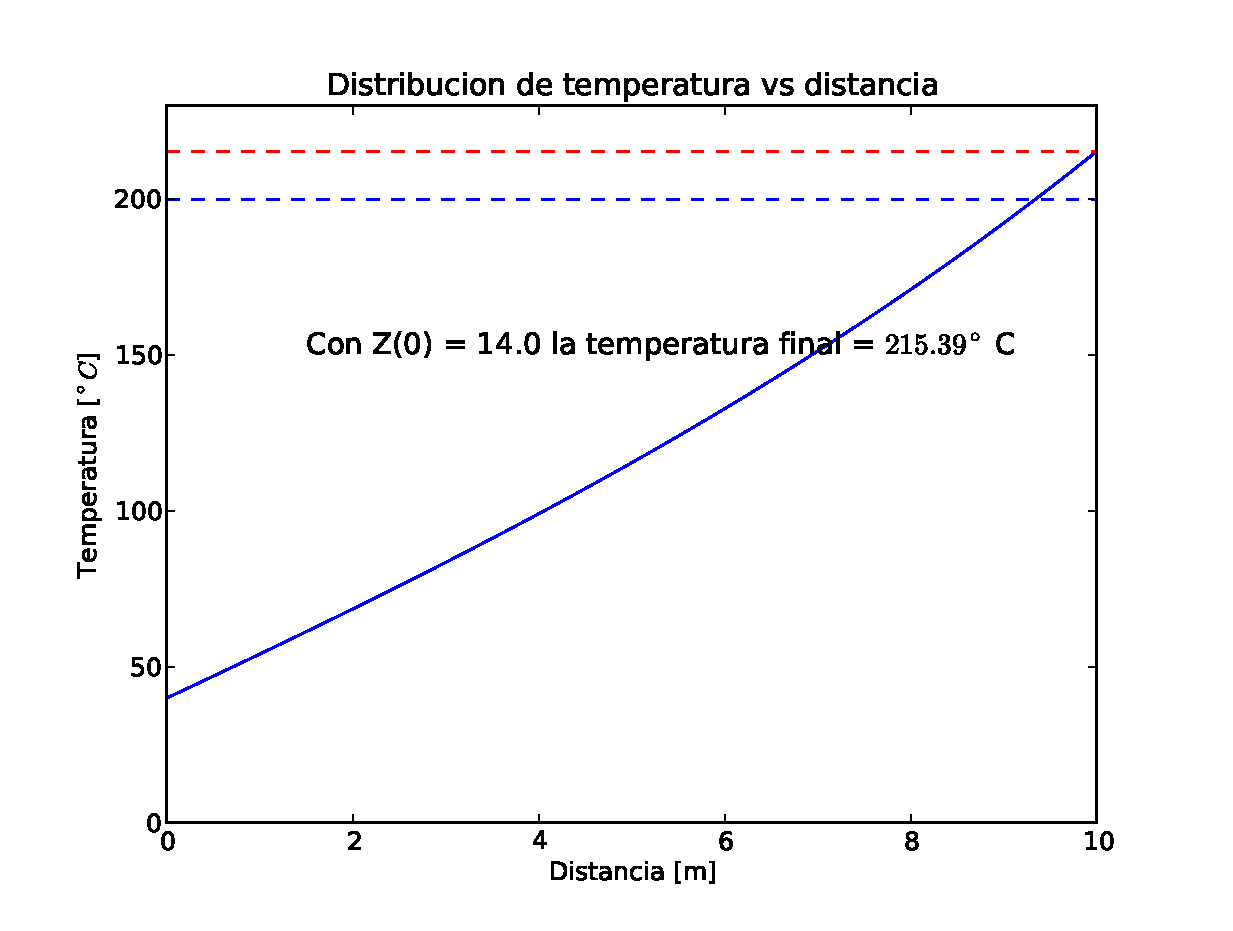
\includegraphics[scale=0.5]{MetDisparo02.eps} 
\end{figure}
\end{frame}
\begin{frame}
Ahora como la EDO original es lineal, los valores
\[ \begin{matrix}
Z(0) = 10 & T(10) = 176.8 \\
Z(0) = 20 & T(10) = 240
\end{matrix} \]
est\'{a}n relacionados linealmente. As\'{i}, podemos usarlos para calcular el valor de $Z(0)$ que resulte para $T(10)=200$.
\\
\bigskip
Podemos usar una f\'{o}rmula de interpolaci\'{o}n lineal
\[ Z(0) =  10 + \dfrac{20-10}{240 - 176.8}(200-176.8) = 13.67 \]
\end{frame}
\begin{frame}
\fontsize{12}{12}\selectfont
\begin{center}
\begin{tabular}{c | c | c}
x & y[0] & y[1] \\ \hline 
0.0000e+00 & 4.0000e+01 & 1.3670e+01 \\
1.0000e+00 & 5.3976e+01 & 1.4272e+01 \\
2.0000e+00 & 6.8526e+01 & 1.4817e+01 \\
3.0000e+00 & 8.3594e+01 & 1.5311e+01 \\
4.0000e+00 & 9.9131e+01 & 1.5757e+01 \\
5.0000e+00 & 1.1509e+02 & 1.6161e+01 \\
6.0000e+00 & 1.3144e+02 & 1.6526e+01 \\
7.0000e+00 & 1.4813e+02 & 1.6857e+01 \\
8.0000e+00 & 1.6514e+02 & 1.7156e+01 \\
9.0000e+00 & 1.8244e+02 & 1.7426e+01 \\
1.0000e+01 & 1.9999e+02 & 1.7671e+01
\end{tabular}
\end{center}
\end{frame}
\begin{frame}
\frametitle{Gr\'{a}ficamente con $Z(0)= 13.67$}
\begin{figure}
	\centering
	\includegraphics[scale=0.5]{MetDisparo03.eps} 
\end{figure}
\end{frame}
\section{Problemas de Sturm-Liouville}
\begin{frame}
Diversos problemas con condiciones en la frontera conducen (mediante el m\'{e}todo de separaci\'{o}n de variables) a la misma ecuaci\'{o}n diferencial ordinaria
\[ X''(x) + \lambda X(x) = 0, \hspace{1cm} (0 < x < L)\]
con el valor propio $\lambda$, pero con distintas condiciones en los extremos:
\begin{enumerate}
\item $X(0) = X(L) = 0$
\item $X'(0) = X'(L) = 0$
\item $X(0) = X'(L) = 0$
\end{enumerate}
seg\'{u}n las condiciones de frontera.
\end{frame}
\begin{frame}
Por ejemplo, en el problema de hallar la temperatura $u(x,t)$ de una varilla $0 \leq x \leq L$ con la temperatura inicial dada $u(x,0)=f(x)$.
\\
\bigskip
Como problema con valores en la frontera, este problema es igual al problema de determinar la temperatura dentro de una l\'{a}mina de gran tamaño que ocupe la regi\'{o}n $0 \leq x \leq L$ en el espacio $xyz$.
\end{frame}
\begin{frame}
Si su temperatura inicial s\'{o}lo depende de $x$ y es independiente de $y$, $z$ (es decir, si $u(x,0)= f(x)$, entonces lo mismo ser\'{a} cierto de su temperatura $u=u(x,y)$ en el instante $t$. Sustituyendo
\[u(x,t) = X(x)T(t)\]
en la ecuaci\'{o}n de calor
\[ \dfrac{\partial u}{\partial t} = k \dfrac{\partial^{2} u}{\partial x^{2}}\]
\end{frame}
\begin{frame}
Vemos que $X(x)$ satisface la condiciones en los extremos, si las caras $x=0$ y $x=L$ de la l\'{a}mina se mantienen a temperatura cero.
\\
\bigskip
Las condiciones de $X'(0) = X'(L) = 0$ si ambas caras est\'{a}n aisladas, y las de $X(0) = X'(L) = 0$, si una cara est\'{a} aislada y la otra se mantiene a temperatura cero.
\end{frame}
\begin{frame}
Pero si cada cara pierde calor hacia el medio ambiente (que se encuentra a temperatura cero) de acuerdo con la ley de enfriamiento de Newton, entonces las condiciones en los extremos asumen la forma
\[h X(0) - X'(0) = 0 = h(X(L) + X'(L)\]
donde $h$ es un coeficiente de transferencia de calor no negativo.
\end{frame}
\begin{frame}
Al imponer diversas condiciones en los extremos sobre la soluci\'{o}n del problema, obtenemos distintos problemas de valores propios, y por ello usamos distintos valores propios ${\lambda_{n}}$ y distintas funciones propioas $X_{n}(x)$ en la construcci\'{o}n de una soluci\'{o}n formal en t\'{e}rminos de una serie de potencias
\[ u(x,t) = \Sigma c_{n} X_{n}(x) T_{n}(x)\]
del problema con valores en la frontera. El paso final en esta construcci\'{o}n es la elecci\'{o}n del coeficiente ${c_{n}}$ en la ecuaci\'{o}n anterior de modo que
\[u(x,0) = \Sigma c_{n} T_{n}(0)X_{n}(x)= f(x) \]
\end{frame}
\begin{frame}
Por lo que necesitamos un desarrollo en t\'{e}rminos de funciones propias de la funci\'{o}n dad $f(x)$, en t\'{e}rminos de las funciones propias del problema con valores en los extremos correspondientes.
\end{frame}
\begin{frame}
\frametitle{Problemas de Sturm-Liouville}
Para unificar y generalizar el m\'{e}todo de separaci\'{o}n de variables, es \'{u}til formular un tipo general de problema de valores propios que incluya como casos particulares a los ya mencionados.
\\
\bigskip
La ecuaci\'{o}n inicial, con $y$ en vez de $X$ como variable dependiente, se puede escribir como
\[ \dfrac{d}{dx} \left[ p(x) \dfrac{dy}{dx} \right] - q(x) y + \lambda r(x) y = 0\]
donde $p(x)=r(x) \equiv 1$ y $q(x) \equiv 0$
\end{frame}
\begin{frame}
Podemos asegurar que casi cualquier ecuaci\'{o}n diferencial lineal de segundo orden de la forma
\[ A(x) y'' + B(x) y' + C(x) y + \lambda D(x) y = 0\]
asume la forma indicada despu\'{e}s de multiplicar por un factor adecuado.
\end{frame}
\begin{frame}
\frametitle{Ejemplo}
Si multiplicamos la ecuaci\'{o}n param\'{e}trica de Bessel de orden $n$
\[ x^{2} y'' + xy' + (\lambda x^{2} - n^{2}) y = 0, \hspace{1cm} x>0\]
por $1/x$, podemos escribir el resultado como
\[ \dfrac{d}{dx} \left[ x \dfrac{dy}{dx} \right] - \dfrac{n^{2}}{x}y + \lambda x y = 0\]
que tiene la forma S-L, con $p(x)=r(x)= x$ y $q(x) = n^{2}/x$
\end{frame}
\begin{frame}
Imponiendo sobre las soluciones de la ecuaci\'{o}n anterior, en un intervalo abierto acotado $(a,b)$ las siguientes condiciones -lineales- homog\'{e}neas en los extremos:
\[ \begin{split}
\alpha_{1} y(a) - \alpha_{2} y'(a) =& 0 \\
\beta_{1} y(b) - \beta_{2} y'(b) =& 0
\end{split} \]
donde los coeficientes $\alpha_{1},\alpha_{2},\beta_{1},\beta_{2}$ son constantes. Adem\'{a}s de ser homog\'{e}neas, las condiciones est\'{a}n \textit{separadas}, en el sentido de que una de ellas implica los valores de $y(x)$ y $y'(x)$ en un extremo $x=a$, mientras que la otra implica los valores en el otro extremo $x=b$. N\'{o}tese que las condiciones $y(a)=y'(b)=0$ son d ela forma dada, con $\alpha_{1}=\beta_{2}=1$ y $\alpha_{2}=\beta_{1}=0$
\end{frame}
\subsection{Definici\'{o}n de un problema Sturm-Liouville}
\begin{frame}
\frametitle{Definici\'{o}n de un problema Sturm-Liouville}
Un problema de Sturm-Liouville es un problema con valores en la frontera de la forma
\[\dfrac{d}{dx} \left[ p(x) \dfrac{dy}{dx} \right] - q(x) y + \lambda r(x) y = 0, \hspace{1cm} a<x<b \]
\[ \begin{split}
\alpha_{1} y(a) - \alpha_{2} y'(a) =& 0 \\
\beta_{1} y(b) - \beta_{2} y'(b) =& 0
\end{split} \]
donde tanto $\alpha_{1}$ y $\alpha_{2}$ como $\beta_{1}$ y $\beta_{2}$ son diferentes de cero. El par\'{a}metro $\lambda$ es el \textit{eingenvalor} cuyos posibles valores (constantes) se buscan.
\end{frame}
\begin{frame}
\frametitle{Ejemplo}
Se obtienen diferentes problemas de Sturm-Liouville complementando la ecuaci\'{o}n diferencial
\[ y'' + \lambda y = 0 \hspace{1cm} 0 < x < L\]
con alguna de las diferentes condiciones de valores en la frontera homog\'{e}neas
\begin{itemize}[<+->]
\item $y(0) = y(L) = 0$, donde $\alpha_{1} = \beta_{1} = 1$ y $\alpha_{2} = \beta_{2} = 0$
\item $y'(0) = y'(L) = 0$, donde $\alpha_{1} = \beta_{1} = 0$ y $\alpha_{2} = \beta_{2} = 1$
\item $y(0) = y'(L) = 0$, donde $\alpha_{1} = \beta_{2} = 1$ y $\alpha_{2} = \beta_{1} = 0$
\end{itemize}
\end{frame}
\begin{frame}
N\'{o}tese que el problema S-L siempre tiene la soluci\'{o}n trivial $y \equiv 0$, por consiguiente se buscan los valores de $\lambda$ (eingenvalores) para los cuales este problema tiene una soluci\'{o}n real \textit{no trivial} (una eigenfunci\'{o}n) y cada eigenvalor cuenta con su eigenfunci\'{o}n asociada (o eigenfunciones).
\\
\bigskip
Puede verse que cualquier constante (diferente de cero) m\'{u}ltiplo de una eigenfunci\'{o}n ser\'{a} tambi\'{e}n una eigenfunci\'{o}n.
\end{frame}
\subsection{Eigenvalores de Sturm-Liouville}
\begin{frame}
\frametitle{Eigenvalores de Sturm-Liouville}
Supongamos que las funciones $p(x), p'(x),q(x)$ y $r(x)$ de la ecuaci\'{o}n S-L son continuas en el intervalo $[a,b]$ y que tanto $p(x)>0$ como $r(x)>0$ en cada punto de $[a,b]$. De este modo los eigenvalores del problema de S-L, constituyen una sucesi\'{o}n creciente
\[ \lambda_{1} < \lambda_{2} < \lambda_{3} < \ldots < \lambda_{n-1} < \lambda_{n} < \ldots\]
de n\'{u}meros reales, con
\[ \lim_{n \rightarrow \infty} \lambda_{n} = + \infty\]
Salvo por un factor constante, solo una eigenfunci\'{o}n $y_{n}(x)$ se asocia con cada eigenvalor $\lambda_{n}$.
\end{frame}
\begin{frame}
Adem\'{a}s, si $q(x) \geq 0$ en $[a,b]$ y los coeficientes $\alpha_{1},\alpha_{2},\beta_{1},\beta_{2}$ en la definici\'{o}n de S-L, son todos no negativos, entonces, los eigenvalores son todos no negativos.
\\
\bigskip
Algunas veces el problema de S-L se llama \textbf{regular} si se satisface el resultado anterior, en caso contrario, es \textbf{singular}.
\end{frame}
\section{Una varilla delgada}
\begin{frame}
\frametitle{Una varilla delgada de metal}
Sea una varilla delgada de metal con longitud $H$, sus extremos est\'{a}n conectados a distintas fuentes de calor:
\begin{center}
\begin{tikzpicture}[font=\small]
\draw [fill=blue!20](0,0) rectangle node {$T_{L}$} (2,4);
\draw (2,1.8) rectangle (3.5,2.2);
\draw (4,1.8) rectangle (5.5,2.2);
\draw [fill=blue!20] (5.5,0) rectangle node {$T_{R}$} (7.5,4);
\draw [<->](2,1.3) -- node [midway, below] {x}(3.5,1.3);
\draw [dashed] (3.5,2.2) -- (3.5,1.25);
\draw [dashed] (4,2.2) -- (4,1.25);
\draw [<-](4,1.3) -- node [midway, below] {dx}(4.6,1.3);
\draw [<->] (2,0.1) -- node [midway, above] {H} (5.5,0.1);
\draw (3.5,4) node {$T_{\infty}$};
\end{tikzpicture}
\end{center}
\end{frame}
\begin{frame}
\fontsize{12}{12}\selectfont
Si el calor sale de la superficie de la varilla \'{u}nicamente por transferencia de calor, por medio de convecci\'{o}n, la ecuaci\'{o}n de temperatura es:
\[ -A \dfrac{d}{dx} k(x) \dfrac{d}{dx} T(x) + h_{c} PT(x) = h_{c} PT_{\infty} + AS(x)\]
donde
\begin{itemize}
\item $T(x)$ es la temperatura del punto que se encuentra a una distancia $x$ del extremo izquierdo.
\item $A$ es el \'{a}rea constante de una secci\'{o}n transversal de la varilla.
\item k es la conductividad t\'{e}rmica.
\item P es el per\'{i}metro de la varilla.
\item $h_{c}$ es el coeficiente de transferencia de calor por convecci\'{o}n.
\item $T_{\infty}$ es la temperatura neta del aire.
\item S es la fuente de calor.
\end{itemize}
\end{frame}
\begin{frame}
Las condiciones de frontera son:
\[ \begin{split} T(0) =& T_{L} \\
T(H) =& T_{R}
\end{split} \]
Si $T^{0}$ se define como:
\[ T^{0} = T - T_{\infty} \]
\end{frame}
\begin{frame}
La ecuaci\'{o}n de temperatura la podemos expresar como:
\[ - \dfrac{d}{dx}k(x) \dfrac{d}{dx} T^{0}(x) + h_{c} \dfrac{P}{A} T^{0}(x) = S(x) \]
El primer t\'{e}rmino representa la difusi\'{o}n del calor, el segundo es la p\'{e}rdida de calor en el aire por medio de la convecci\'{o}n y el lado derecho es la fuente de calor.
\end{frame}
\begin{frame}
Otro ejemplo de una EDO con forma similar es la ecuaci\'{o}n de difusi\'{o}n de neutrones dada por:
\[ - \dfrac{d}{dx} D(x) \dfrac{d}{dx} \Psi (x) + \Sigma_{a} \Psi (x) = S(x) \]
Donde $\Psi$ es el flujo de neutrones, $D$ es el coeficiente de difusi\'{o}n y $S$ es la fuente de neutrones.
\\
\bigskip
El primer t\'{e}rmino indica la difusi\'{o}n de neutrones, el segundo la p\'{e}rdida por absorci\'{o}n y el lado derecho es la fuente de neutrones.
\end{frame}
\begin{frame}
Considerando en otros casos dentro de la f\'{i}sica para problemas con difusi\'{o}n, si se expresa en t\'{e}rminos de:
\[- \dfrac{d}{dx} p(x) \dfrac{d}{dx} \phi (x) + q(x) \phi (x) = S(x)  \]
siendo \'{e}sta, una ley de conservaci\'{o}n de la difusi\'{o}n.
\end{frame}
\begin{frame}
Integrando la ecuaci\'{o}n anterior en el intervalo $[a,b]$, se obtiene que:
\[ Z(b) - Z(a) + \int_{b}^{a} q(x) \phi (x) dx = \int_{b}^{a} S(x) dx \]
donde
\[ Z(x) = - p(x) \dfrac{d}{dx} \phi (x) \]
\end{frame}
\subsection{Problemas con valores en la frontera para varillas y l\'{a}minas}
\begin{frame}
\frametitle{Problemas con valores en la frontera para varillas y l\'{a}minas}
Consideremos una EDO de segundo orden con valores en la frontera
\[ - \phi'' (x) + q \phi (x) = S(x), \hspace{1cm} 0< x < H \]
con condiciones de frontera:
\begin{itemize}
\item $\phi'(0) = 0$, condici\'{o}n de frontera izquierda.
\item $\phi'(H) = \phi'_{R}$, condici\'{o}n de frontera derecha
\end{itemize}
\end{frame}
\begin{frame}
Si dividimos el dominio en $N$ intervalos de igual longitud, se obtiene una ret\'{i}cula donde los intervalos miden $h = H/N$
\begin{center}
\begin{tikzpicture}[font=\small]
\draw (0,1) node {$\phi'=0$};
\draw (7,1) node {$\phi'=\phi_{R}$};
\draw (-1.3,0) -- (8,0);
\foreach \x in {-1,...,7}
	\draw [fill=red!25](\x,0) circle (0.05);
\draw (-1.3,-0.5) node {x=-h};
\draw (0,-0.5) node {0};
\draw (1,-0.5) node {h};
\draw (2,-0.5) node {2h};
\draw (3,-0.5) node {3h};
\draw (7,-0.5) node {Nh=H};
\draw (-1.3,-1) node {i=0};
\draw (0,-1) node {1};
\draw (1,-1) node {2};
\draw (2,-1) node {3};
\draw (3,-1) node {4};
\draw (6,-1) node {N};
\draw (7,-1) node {N=N+1};
\end{tikzpicture}
\end{center}
\end{frame}
\begin{frame}
Usando una aproximaci\'{o}n por diferencias centrales al primer t\'{e}rmino de la EDO de segundo orden, obtenemos la ecuaci\'{o}n en diferencias para
la $i$-\'{e}sima ret\'{i}cula:
\[ \dfrac{(-\phi_{i-1} + 2 \phi_{i} - \phi_{i+1})}{h^{2}} + q \phi_{i} = S_{i} \]
donde $\phi_{i}=\phi(x_{i})$, $S_{i}=S(x_{i})$ y $q$ es constante.
\end{frame}
\begin{frame}
Al multiplicar por $h^{2}$
\[ - \phi_{i-1} + (2-w) \phi_{i} - \phi_{i+1} = h^{2}S_{i} \]
donde $w=qh^{2}$.
\\
\bigskip
Esta ecuaci\'{o}n se puede aplicar a todos los puntos de la ret\'{i}cula, excepto cuando $i = 1$ e $i = N+1$.
\end{frame}
\begin{frame}
La condici\'{o}n de la frontera izquierda $\phi'(0) = 0$, es equivalente a una condici\'{o}n sim\'{e}trica en la frontera llamada condici\'{o}n adiab\'{a}tica en la frontera en el caso de la transferencia de calor.
\\
\bigskip
Si se considera un punto hipot\'{e}tico de la ret\'{i}cula $i = 0$ localizado en $x = -h$, la ecuaci\'{o}n anterior en el caso $i = 1$ es:
\[-\phi_{0} + (2+w)\phi_{1} - \phi_{2} = h^{2}S_{1} \]
\end{frame}
\begin{frame}
En esta ecuaci\'{o}n
\[-\phi_{0} + (2+w)\phi_{1} - \phi_{2} = h^{2}S_{1} \]
podemos hacer $\phi_{0} = \phi_{2}$ debido a la simetr\'{i}a. Dividiendo entre dos, obtenemos lo siguiente:
\[ (1 + \dfrac{w}{2}) \phi_{1} - \phi_{2} = \dfrac{1}{2} h^{2}S_{1}\]
como $\phi_{N+1}= \phi(H)=\phi_{R}$ en la frontera derecha, la ecuaci\'{o}n con $i=N$ es:
\[ -\phi_{N+1} + (2+w) \phi_{N} = h^{2}S_{N} + \phi_{R}\]
\end{frame}
\begin{frame}
Ordenando los t\'{e}rminos anteriores:
%\fontsize{10}{10}\selectfont
\[ \tiny{\begin{matrix}
(1+\frac{w}{2})\phi_{1} & -\phi_{2}      &                &           &            & & = h^{2}\frac{S_{1}}{2} \\
-\phi_{1}               & +(2+w)\phi_{2} & -\phi_{3}      &           &            & & = h^{2}S_{2} \\
                        & \phi_{2}       & +(2+w)\phi_{3} & -\phi_{4} &            & & = h^{2}S_{3} \\
                        &                &                &           &            & & \ldots \\
                        &                &                &           &            & & \ldots \\
                        &                &                &           &-\phi_{N+1} & +(2+w)\phi_{N} & = h^{2}S_{N}+\phi_{R} 
\end{matrix}} \]
\end{frame}
\begin{frame}
Que en forma matricial, resulta
\fontsize{10}{10}\selectfont
\[ \small{\begin{bmatrix}
1+w/2 & -1 & 0 & 0 & 0 & 0 \\
-1 & 2+w & -1 & 0 & 0 & 0 \\
0 & -1 & 2+w & -1 & 0 & 0 \\
0 & 0 & 0 + \ddots & -1 & 0 & 0 \\
0 & 0 & 0 & 0 & -1 & 2+w
\end{bmatrix} 
\begin{bmatrix}
\phi_{1} \\
\phi_{2} \\
\phi_{3} \\
\ddots \\
\phi_{N} \\
\end{bmatrix} =
\begin{bmatrix}
h^{2}S_{1}/2 \\
h^{2}S_{2} \\
h^{2}S_{3} \\
\ddots \\
h^{2}S_{N}+\phi_{R} \\
\end{bmatrix}}
\]
\end{frame}
\subsection{Soluci\'{o}n de sistemas tridiagonales}
\begin{frame}
\frametitle{Soluci\'{o}n de sistemas tridiagonales}
Una ecuaci\'{o}n tridiagonal la podemos escribir de la siguiente forma:
\[
\begin{bmatrix}
B_{1} & C_{1} & 0 & 0 & 0 & 0 \\
A_{2} & B_{2} & C_{2} & 0 & 0 & 0 \\
0 & A_{3} & B_{3} & C_{3} & 0 & 0 \\
0 & 0 & 0 & \ddots & 0 & 0 \\
0 & 0 & 0 & 0 & A_{n}& B_{n} 
\end{bmatrix}
\begin{bmatrix}
\phi_{1} \\
\phi_{2} \\
\phi_{3} \\
\ddots \\
\phi_{N} \\
\end{bmatrix} =
\begin{bmatrix}
D_{1} \\
D_{2} \\
D_{3} \\
\ddots \\
D_{N} \\
\end{bmatrix}
\]
\end{frame}
\begin{frame}
El algoritmo de soluci\'{o}n para esta matriz es el siguiente:
\begin{enumerate}
\item Se inicializan dos nuevas variables: $B'_{1}=B_{1}$ y $D'_{1}=D_{1}$.
\item Se calculan de forma recursiva las siguientes ecuaciones, de $i$ hasta $N$:
\[ \begin{split} R &= \dfrac{A_{i}}{B'_{i-1}} \\
B'_{i} &= B_{i} -RC_{i-1} \\
D'_{i} &= D_{i} - RD'_{i-1}, \hspace{1cm} i=2,3,\ldots,N
\end{split} \]
\end{enumerate}
\end{frame}
\begin{frame}
\begin{enumerate}
\setcounter{enumi}{2}
\item Se calcula la soluci\'{o}n para la \'{u}ltima inc\'{o}gnita
\[ \phi_{i} = \dfrac{(D'_{i}-C_{i}\phi_{i+1})}{B'_{i}}, \hspace{1.5 cm} i=N-1, N-2,\ldots,1\]
\end{enumerate}
\end{frame}
\begin{frame}
\frametitle{Ejercicio}
Determinar las ecuaciones en diferencias y su soluci\'{o}n para el siguiente problema con valores en la frontera:
\[ -2y''(x) + y(x) = e^{-0.2x} \]
con las condiciones de frontera
\[ \begin{split} 
y(0) &= 1 \\
y'(10) &= -y(10)
\end{split} \]
Supongamos que los intervalos de la ret\'{i}cula tienen longitud unitaria.
\end{frame}
\begin{frame}
\frametitle{Soluci\'{o}n}
En la siguiente figura se muestra la ret\'{i}cula
\begin{center}
\begin{tikzpicture}[font=\small]
\draw (-1.3,0) -- (8,0);
\foreach \x in {-1,...,7}
	\draw [fill=red!25](\x,0) circle (0.05);
\draw (-1.3,-0.5) node {x=0};
\draw (0,-0.5) node {1};
\draw (1,-0.5) node {2};
\draw (6,-0.5) node {9};
\draw (7,-0.5) node {x=10};
\draw (-1.3,-1) node {i=0};
\draw (0,-1) node {1};
\draw (1,-1) node {2};
\draw (6,-1) node {9};
\draw (7,-1) node {10};
\end{tikzpicture}
\end{center}
Las ecuaciones en diferencias para $i=1$ hasta $i=9$, son:
\[ 2(-y_{i-1}+2y_{i}-y_{i+1}) + y_{i} = e^{-0.2i}, \hspace{1cm} x_{i}=i \]
\end{frame}
\begin{frame}
Para $i=1$, sustituimos la condici\'{o}n de frontera $y_{0}=y(0)=1$ en las ecuaciones anteriores, y resulta que:
\[ 5y_{1}-2y_{2} = e^{-0.2} +2\]
Para $i=10$, aproximamos la ecuaci\'{o}n diferencial por:
\[ - \dfrac{2(y'(10)- y'(9.5))}{\frac{1}{2}} + y(10) = e^{-2}\]
\end{frame}
\begin{frame}
Por medio de la aproximaci\'{o}n por diferencias centrales, el t\'{e}rmino $y'(9.5)$ es
\[ y'(9.5) = \dfrac{y(10)-y(9)}{1}\]
Sustituimos el resultado anterior y la condici\'{o}n de frontera $y'(10)=-y(10)$, para obtener
\[ -2y_{9} + 4.5y_{10} =  0.5 e^{-2} \]
\end{frame}
\begin{frame}
Las ecuaciones en diferencias son entonces
\[ \begin{split}
5y_{1} - 2y_{2} &= e^{-0.2} +2 \\
-2y_{i-1} + 5y_{i} - 2y_{i+1} &= e^-0.2x_{i}, \hspace{1cm} i=2,\ldots,9 \\
-2y_{9} + 4.5 y_{10} &= 0.5 e^{-2}
\end{split} \]
Donde $x_{i}=i$
\end{frame}
\begin{frame}
La matriz tridiagonal es
\[ \tiny{\begin{bmatrix}
5 & -2 & 0 & 0 & 0 & 0 & 0 & 0 & 0 & 0 \\
-2 & 5 & -2 & 0 & 0 & 0 & 0 & 0 & 0 & 0 \\
0 & -2 & 5 & -2 & 0 & 0 & 0 & 0 & 0 & 0 \\
0 & 0 & -2 & 5 & -2 & 0 & 0 & 0 & 0 & 0 \\
0 & 0 & 0 & -2 & 5 & -2 & 0 & 0 & 0 & 0 \\
0 & 0 & 0 & 0& -2 & 5 & -2 & 0 & 0 & 0 \\
0 & 0 & 0 & 0 & 0 & -2 & 5 & -2 & 0 & 0 \\
0 & 0 & 0 & 0 & 0 & 0 & -2 & 5 & -2 & 0 \\
0 & 0 & 0 & 0 & 0 & 0 & 0 & -2 & 5 & -2 \\
0 & 0 & 0 & 0 & 0 & 0 & 0 & 0 & -2 & 4.5 
\end{bmatrix}
\begin{bmatrix}
y_{1} \\
y_{2} \\
y_{3} \\
y_{4} \\
y_{5} \\
y_{6} \\
y_{7} \\
y_{8} \\
y_{9} \\
y_{10} \\
\end{bmatrix} =
\begin{bmatrix}
e^{-0.2}+2 \\
e^{-0.2x_{2}} \\
e^{-0.2x_{3}} \\
e^{-0.2x_{4}} \\
e^{-0.2x_{5}} \\
e^{-0.2x_{6}} \\
e^{-0.2x_{7}} \\
e^{-0.2x_{8}} \\
e^{-0.2x_{9}} \\
0.5e^{-2}
\end{bmatrix}} \]
\end{frame}
\begin{frame}
\frametitle{Soluci\'{o}n}
Implementando el c\'{o}digo en Python, tenemos los siguientes valores
\\
\medskip
\begin{minipage}{4cm}
\begin{tabular}{c | c}
ret\'{i}cula & soluci\'{o}n \\ \hline
0 & 1.00000000 \\
1 & 0.84643489 \\
2 & 0.70672186 \\
3 & 0.58520973 \\
4 & 0.48189665 \\
5 & 0.39486742 \\
\end{tabular}
\end{minipage}
\hspace{0.5cm}
\begin{minipage}{4cm}
\begin{tabular}{c | c}
ret\'{i}cula & soluci\'{o}n \\ \hline
6 & 0.32133217 \\
7 & 0.25786591 \\
8 & 0.20003411 \\
9 & 0.14127111 \\
10 & 0.07049423 \\
 & 
\end{tabular}
\end{minipage}
\end{frame}
\end{document}